% GENERATED FILE - do not hand-edit.
% Source of truth: data/calculus-reviewed/c-9.json in the zenith-website repo.
% Regenerate with: python3 scripts/build_calculus_tex.py
\documentclass[11pt]{article}
\usepackage[utf8]{inputenc}
\usepackage[T1]{fontenc}
\usepackage{amsmath,amssymb}
\usepackage{graphicx}
\usepackage[margin=1in]{geometry}
\graphicspath{{../..//}}
\setlength{\parindent}{0pt}
\setlength{\parskip}{0.6em}
\begin{document}
\section*{Chapter 9: Differential Equations --- Practice Exercises C9}

\bigskip\noindent\textbf{A1.}\ Acceleration is $a(t)=4t-1$ and velocity satisfies $v(1)=3$. Find $v(t)$.
\begin{list}{}{\setlength{\leftmargin}{3em}\setlength{\labelwidth}{2.5em}\setlength{\itemsep}{0pt}\setlength{\topsep}{2pt}}
\item[(A)] $2t^2-t$
\item[(B)] $2t^2-t+1$
\item[(C)] $2t^2-t+2$
\item[(D)] $2t^2+1$
\end{list}

\bigskip\noindent\textbf{A2.}\ Acceleration is $a(t)=20t^3-6t$, and position satisfies $s(-1)=2$, $s(1)=4$. Find velocity $v(t)$.
\begin{list}{}{\setlength{\leftmargin}{3em}\setlength{\labelwidth}{2.5em}\setlength{\itemsep}{0pt}\setlength{\topsep}{2pt}}
\item[(A)] $5t^4-3t^2+1$
\item[(B)] $5t^4-3t^2+3$
\item[(C)] $t^5-t^3+t+3$
\item[(D)] $t^5-t^3+1$
\end{list}

\bigskip\noindent\textbf{A3.}\ Acceleration is $a(t)=20t^3-6t$, and position satisfies $s(-1)=2$, $s(1)=4$. Find $s(0)$.
\begin{list}{}{\setlength{\leftmargin}{3em}\setlength{\labelwidth}{2.5em}\setlength{\itemsep}{0pt}\setlength{\topsep}{2pt}}
\item[(A)] $1$
\item[(B)] $2$
\item[(C)] $3$
\item[(D)] $4$
\end{list}

\bigskip\noindent\textbf{A4.}\ A stone is thrown upward from a building at 40 ft/sec and hits the ground 4 seconds later. With gravity $-32$ ft/sec$^2$, find the building height in feet.
\begin{list}{}{\setlength{\leftmargin}{3em}\setlength{\labelwidth}{2.5em}\setlength{\itemsep}{0pt}\setlength{\topsep}{2pt}}
\item[(A)] $88$
\item[(B)] $96$
\item[(C)] $112$
\item[(D)] $128$
\end{list}

\bigskip\noindent\textbf{A5.}\ A stone is thrown upward from a building at 40 ft/sec and hits the ground 4 seconds later. With gravity $-32$ ft/sec$^2$, when does it reach maximum height?
\begin{list}{}{\setlength{\leftmargin}{3em}\setlength{\labelwidth}{2.5em}\setlength{\itemsep}{0pt}\setlength{\topsep}{2pt}}
\item[(A)] $4/5$ second
\item[(B)] $4$ seconds
\item[(C)] $5/4$ seconds
\item[(D)] $2$ seconds
\end{list}

\bigskip\noindent\textbf{A6.}\ A car accelerates constantly from 0 to 60 mph in 10 seconds. Given 60 mph = 88 ft/sec, find distance traveled.
\begin{list}{}{\setlength{\leftmargin}{3em}\setlength{\labelwidth}{2.5em}\setlength{\itemsep}{0pt}\setlength{\topsep}{2pt}}
\item[(A)] $44$ feet
\item[(B)] $88$ feet
\item[(C)] $400$ feet
\item[(D)] $440$ feet
\end{list}

\bigskip\noindent\textbf{A7.}\ A stone has velocity $v(t)=100-20t$ ft/sec and hits a target at $t=1$ second. Find distance from sling to target.
\begin{list}{}{\setlength{\leftmargin}{3em}\setlength{\labelwidth}{2.5em}\setlength{\itemsep}{0pt}\setlength{\topsep}{2pt}}
\item[(A)] $80$ feet
\item[(B)] $90$ feet
\item[(C)] $100$ feet
\item[(D)] $110$ feet
\end{list}

\bigskip\noindent\textbf{A8.}\ A stone is thrown vertically from the ground. With gravity $-32$ ft/sec$^2$, what initial velocity gives a maximum height of 100 feet?
\begin{list}{}{\setlength{\leftmargin}{3em}\setlength{\labelwidth}{2.5em}\setlength{\itemsep}{0pt}\setlength{\topsep}{2pt}}
\item[(A)] $50$ ft/sec
\item[(B)] $80$ ft/sec
\item[(C)] $92$ ft/sec
\item[(D)] $96$ ft/sec
\end{list}

\bigskip\noindent\textbf{A9.}\ If the velocity of a car traveling in a straight line at time $t$ is $v(t)$, then the difference in its odometer readings between times $t=a$ and $t=b$ is
\begin{list}{}{\setlength{\leftmargin}{3em}\setlength{\labelwidth}{2.5em}\setlength{\itemsep}{0pt}\setlength{\topsep}{2pt}}
\item[(A)] $\displaystyle\int_a^b |v(t)|\,dt$
\item[(B)] $\displaystyle\int_a^b v(t)\,dt$
\item[(C)] the net displacement of the car's position from $t=a$ to $t=b$
\item[(D)] the change in the car's position from $t=a$ to $t=b$
\end{list}

\bigskip\noindent\textbf{A10.}\ If an object is moving up and down along the $y$-axis with velocity $v(t)$ and $s'(t)=v(t)$, then it is false that $\displaystyle\int_a^b v(t)\,dt$ gives
\begin{list}{}{\setlength{\leftmargin}{3em}\setlength{\labelwidth}{2.5em}\setlength{\itemsep}{0pt}\setlength{\topsep}{2pt}}
\item[(A)] $s(b)-s(a)$
\item[(B)] the total change in $s(t)$ between $t=a$ and $t=b$
\item[(C)] the shift in the object's position from $t=a$ to $t=b$
\item[(D)] the total distance covered by the object from $t=a$ to $t=b$
\end{list}

\bigskip\noindent\textbf{A11.}\ Solutions of $dy/dx=x/y$ have the form
\begin{list}{}{\setlength{\leftmargin}{3em}\setlength{\labelwidth}{2.5em}\setlength{\itemsep}{0pt}\setlength{\topsep}{2pt}}
\item[(A)] $x^2-y^2=C$
\item[(B)] $x^2+y^2=C$
\item[(C)] $x^2-Cy^2=0$
\item[(D)] $x^2=C-y^2$
\end{list}

\bigskip\noindent\textbf{A12.}\ Find the domain of the particular solution of $dy/dx=x/y$ through $(-2,1)$.
\begin{list}{}{\setlength{\leftmargin}{3em}\setlength{\labelwidth}{2.5em}\setlength{\itemsep}{0pt}\setlength{\topsep}{2pt}}
\item[(A)] $x<0$
\item[(B)] $-2\le x<0$
\item[(C)] $x<-\sqrt3$
\item[(D)] $|x|>\sqrt3$
\end{list}

\bigskip\noindent\textbf{A13.}\ If $dy/dx=y/(2\sqrt x)$ and $y(4)=1$, then
\begin{list}{}{\setlength{\leftmargin}{3em}\setlength{\labelwidth}{2.5em}\setlength{\itemsep}{0pt}\setlength{\topsep}{2pt}}
\item[(A)] $\ln y=4\sqrt x-8$
\item[(B)] $\ln y=\sqrt{x-2}$
\item[(C)] $y=e^{\sqrt x}$
\item[(D)] $y=e^{\sqrt x-2}$
\end{list}

\bigskip\noindent\textbf{A14.}\ If $dy/dx=e^y$ and $y(1)=0$, then
\begin{list}{}{\setlength{\leftmargin}{3em}\setlength{\labelwidth}{2.5em}\setlength{\itemsep}{0pt}\setlength{\topsep}{2pt}}
\item[(A)] $y=\ln x$
\item[(B)] $y=\ln(2-x)$
\item[(C)] $y=-\ln(2-x)$
\item[(D)] $y=-\ln x$
\end{list}

\bigskip\noindent\textbf{A15.}\ If $dy/dx=x/\sqrt{9+x^2}$ and $y(4)=5$, find $y$.
\begin{list}{}{\setlength{\leftmargin}{3em}\setlength{\labelwidth}{2.5em}\setlength{\itemsep}{0pt}\setlength{\topsep}{2pt}}
\item[(A)] $\sqrt{9+x^2}-5$
\item[(B)] $\sqrt{9+x^2}$
\item[(C)] $(\sqrt{9+x^2}+5)/2$
\item[(D)] $\sqrt{9+x^2}/2$
\end{list}

\bigskip\noindent\textbf{A16.}\ The general solution of $x\,dy=y\,dx$ is a family of
\begin{list}{}{\setlength{\leftmargin}{3em}\setlength{\labelwidth}{2.5em}\setlength{\itemsep}{0pt}\setlength{\topsep}{2pt}}
\item[(A)] circles
\item[(B)] hyperbolas
\item[(C)] parabolas
\item[(D)] none of these
\end{list}

\bigskip\noindent\textbf{A17.}\ The general solution of $dy/dx=y$ is a family of
\begin{list}{}{\setlength{\leftmargin}{3em}\setlength{\labelwidth}{2.5em}\setlength{\itemsep}{0pt}\setlength{\topsep}{2pt}}
\item[(A)] parabolas
\item[(B)] lines
\item[(C)] ellipses
\item[(D)] exponential curves
\end{list}

\bigskip\noindent\textbf{A18.}\ Find $f$ satisfying $f(x)f'(x)=x$ and $f(0)=1$.
\begin{list}{}{\setlength{\leftmargin}{3em}\setlength{\labelwidth}{2.5em}\setlength{\itemsep}{0pt}\setlength{\topsep}{2pt}}
\item[(A)] $\sqrt{x^2+1}$
\item[(B)] $\sqrt{1-x^2}$
\item[(C)] $x$
\item[(D)] $e^x$
\end{list}

\bigskip\noindent\textbf{A19.}\ A curve passes through $(1,1)$ and satisfies $dy/dx=3y/x$. Its equation is
\begin{list}{}{\setlength{\leftmargin}{3em}\setlength{\labelwidth}{2.5em}\setlength{\itemsep}{0pt}\setlength{\topsep}{2pt}}
\item[(A)] $3x-2=y$
\item[(B)] $y^3=x$
\item[(C)] $y=x^3$
\item[(D)] $3y^2=x^2+2$
\end{list}

\bigskip\noindent\textbf{A20.}\ Find the domain of the particular solution of $dy/dx=3y/x$ through $(1,1)$.
\begin{list}{}{\setlength{\leftmargin}{3em}\setlength{\labelwidth}{2.5em}\setlength{\itemsep}{0pt}\setlength{\topsep}{2pt}}
\item[(A)] all real numbers
\item[(B)] $|x|\le1$
\item[(C)] $x\ne0$
\item[(D)] $x>0$
\end{list}

\bigskip\noindent\textbf{A21.}\ If $dy/dx=k/x$, $y(1)=2$, and $y(e)=4$, what is $y(2)$?
\begin{list}{}{\setlength{\leftmargin}{3em}\setlength{\labelwidth}{2.5em}\setlength{\itemsep}{0pt}\setlength{\topsep}{2pt}}
\item[(A)] $4$
\item[(B)] $\ln8$
\item[(C)] $\ln2+2$
\item[(D)] $\ln4+2$
\end{list}

\bigskip\noindent\textbf{A22.}\ Which differential equation has the displayed slope field on $[-2\pi,2\pi]\times[-1.5,1.5]$?
\begin{center}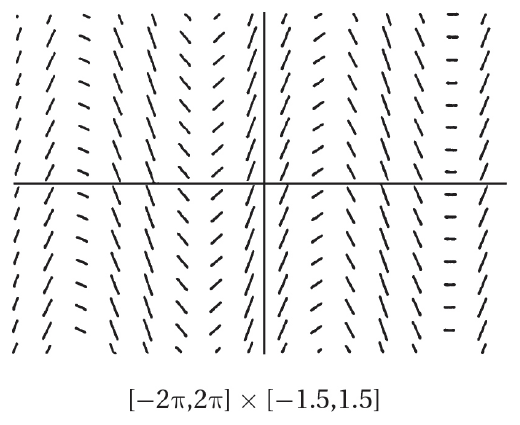
\includegraphics[width=0.6\linewidth]{data/calculus-figures/c9-a22.png}\end{center}
\begin{list}{}{\setlength{\leftmargin}{3em}\setlength{\labelwidth}{2.5em}\setlength{\itemsep}{0pt}\setlength{\topsep}{2pt}}
\item[(A)] $\dfrac{dy}{dx}=\sin x$
\item[(B)] $\dfrac{dy}{dx}=-\sin x$
\item[(C)] $\dfrac{dy}{dx}=\cos x$
\item[(D)] $\dfrac{dy}{dx}=-\cos x$
\end{list}

\bigskip\noindent\textbf{A23.}\ Which equation has the displayed slope field on $[-5,5]\times[-3,3]$?
\begin{center}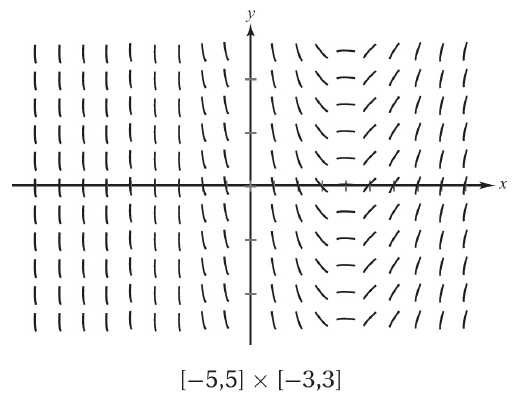
\includegraphics[width=0.6\linewidth]{data/calculus-figures/c9-a23.png}\end{center}
\begin{list}{}{\setlength{\leftmargin}{3em}\setlength{\labelwidth}{2.5em}\setlength{\itemsep}{0pt}\setlength{\topsep}{2pt}}
\item[(A)] $y'=2x$
\item[(B)] $y'=2x-4$
\item[(C)] $y'=4-2x$
\item[(D)] $y'=y$
\end{list}

\bigskip\noindent\textbf{A24.}\ A solution curve has been superimposed on the slope field shown above. The solution is for the differential equation and initial condition
\begin{center}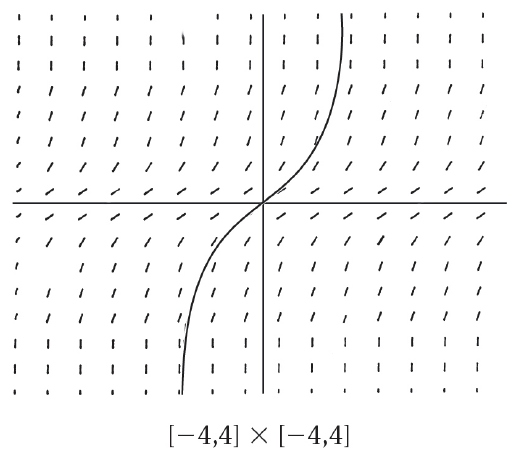
\includegraphics[width=0.6\linewidth]{data/calculus-figures/c9-a24.png}\end{center}
\begin{list}{}{\setlength{\leftmargin}{3em}\setlength{\labelwidth}{2.5em}\setlength{\itemsep}{0pt}\setlength{\topsep}{2pt}}
\item[(A)] $\dfrac{dy}{dx}=\tan x$; $y(0)=0$
\item[(B)] $\dfrac{dy}{dx}=1+x^2$; $y(0)=0$
\item[(C)] $\dfrac{dy}{dx}=\dfrac{1}{1+x^2}$; $y\left(\dfrac{\pi}{4}\right)=1$
\item[(D)] $\dfrac{dy}{dx}=1+y^2$; $y(0)=0$
\end{list}

\bigskip\noindent\textbf{A25.}\ Which displayed slope field represents $dy/dx=y$?
\begin{center}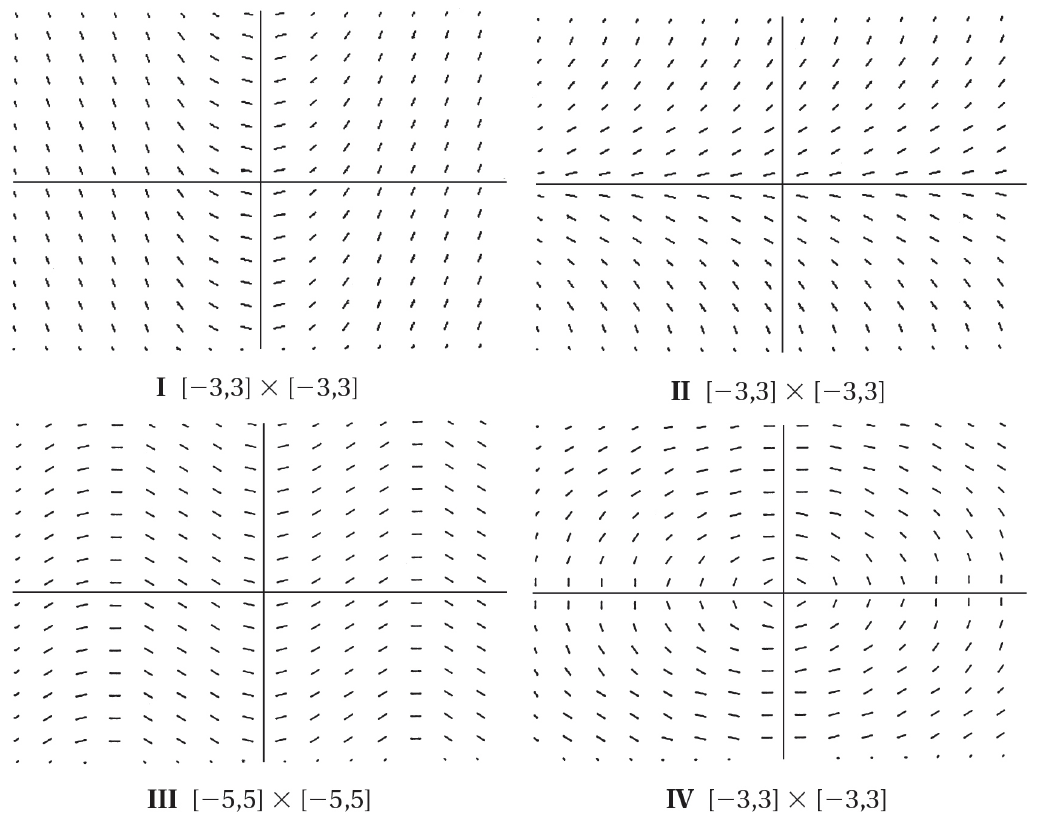
\includegraphics[width=0.6\linewidth]{data/calculus-figures/c9-a25-a29.png}\end{center}
\begin{list}{}{\setlength{\leftmargin}{3em}\setlength{\labelwidth}{2.5em}\setlength{\itemsep}{0pt}\setlength{\topsep}{2pt}}
\item[(A)] I
\item[(B)] II
\item[(C)] III
\item[(D)] IV
\end{list}

\bigskip\noindent\textbf{A26.}\ Which displayed slope field represents $dy/dx=-x/y$?
\begin{center}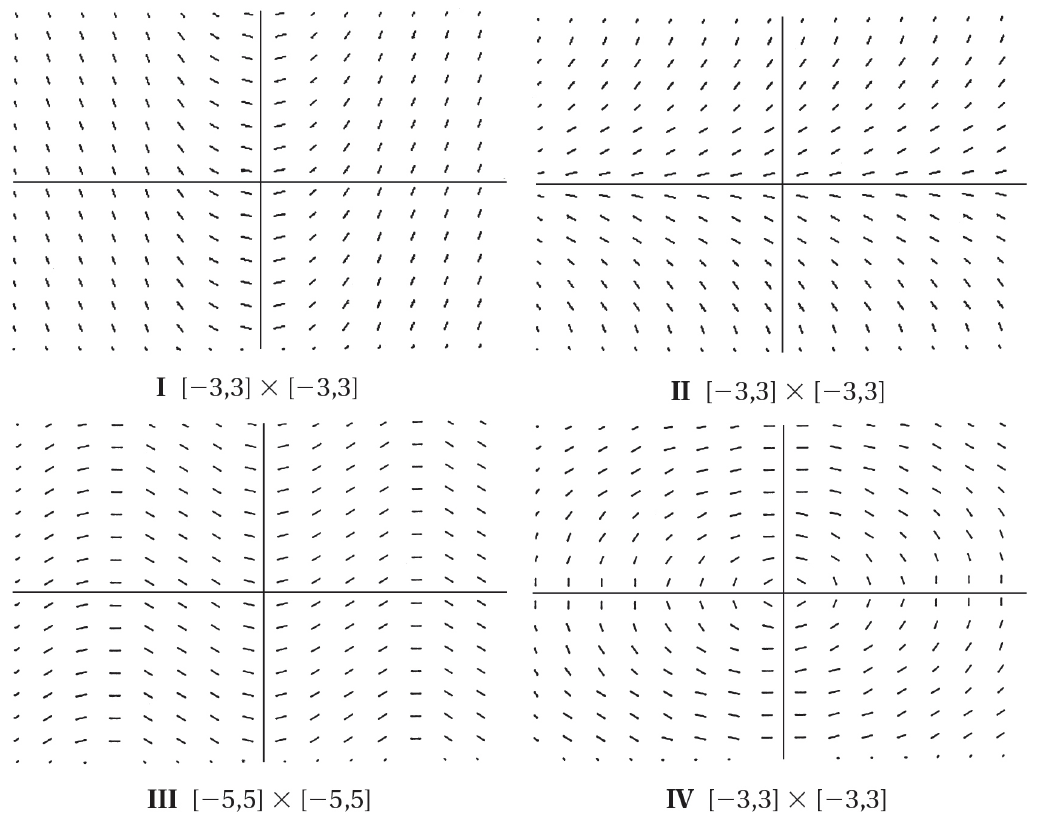
\includegraphics[width=0.6\linewidth]{data/calculus-figures/c9-a25-a29.png}\end{center}
\begin{list}{}{\setlength{\leftmargin}{3em}\setlength{\labelwidth}{2.5em}\setlength{\itemsep}{0pt}\setlength{\topsep}{2pt}}
\item[(A)] I
\item[(B)] II
\item[(C)] III
\item[(D)] IV
\end{list}

\bigskip\noindent\textbf{A27.}\ Which displayed slope field represents $dy/dx=\sin x$?
\begin{center}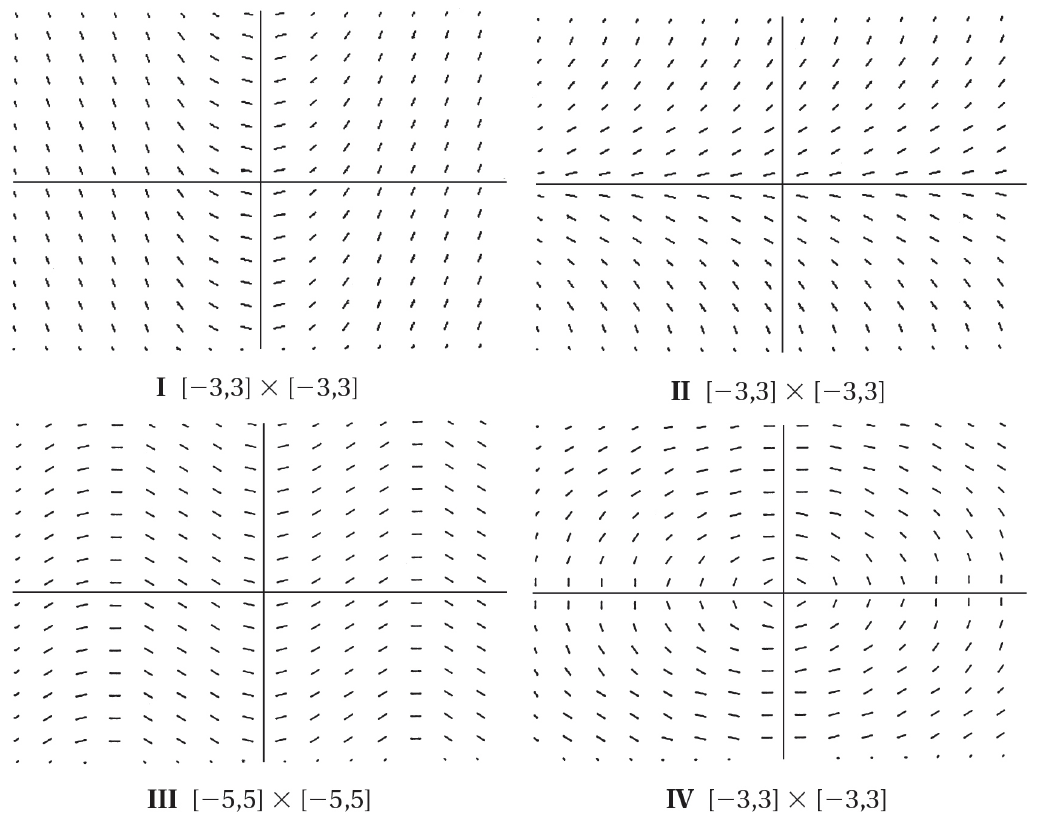
\includegraphics[width=0.6\linewidth]{data/calculus-figures/c9-a25-a29.png}\end{center}
\begin{list}{}{\setlength{\leftmargin}{3em}\setlength{\labelwidth}{2.5em}\setlength{\itemsep}{0pt}\setlength{\topsep}{2pt}}
\item[(A)] I
\item[(B)] II
\item[(C)] III
\item[(D)] IV
\end{list}

\bigskip\noindent\textbf{A28.}\ Which displayed slope field represents $dy/dx=2x$?
\begin{center}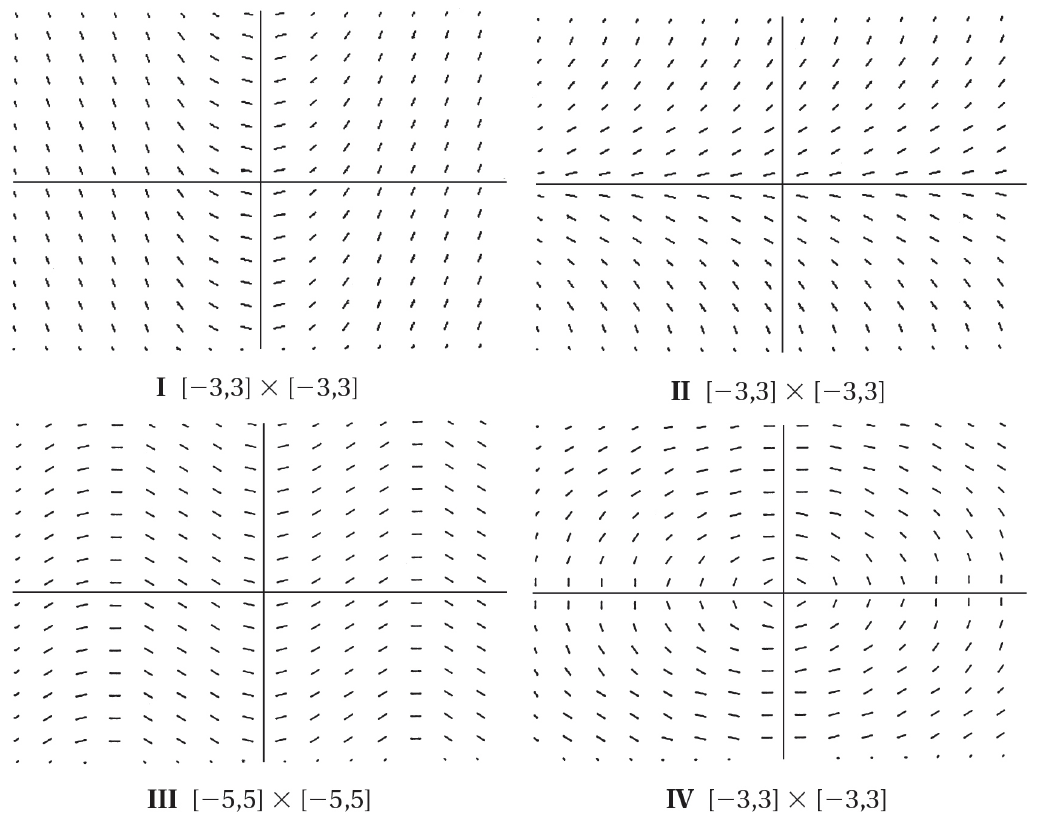
\includegraphics[width=0.6\linewidth]{data/calculus-figures/c9-a25-a29.png}\end{center}
\begin{list}{}{\setlength{\leftmargin}{3em}\setlength{\labelwidth}{2.5em}\setlength{\itemsep}{0pt}\setlength{\topsep}{2pt}}
\item[(A)] I
\item[(B)] II
\item[(C)] III
\item[(D)] IV
\end{list}

\bigskip\noindent\textbf{A29.}\ The solution represented by field II passes through $(0,-1)$. Its equation is
\begin{center}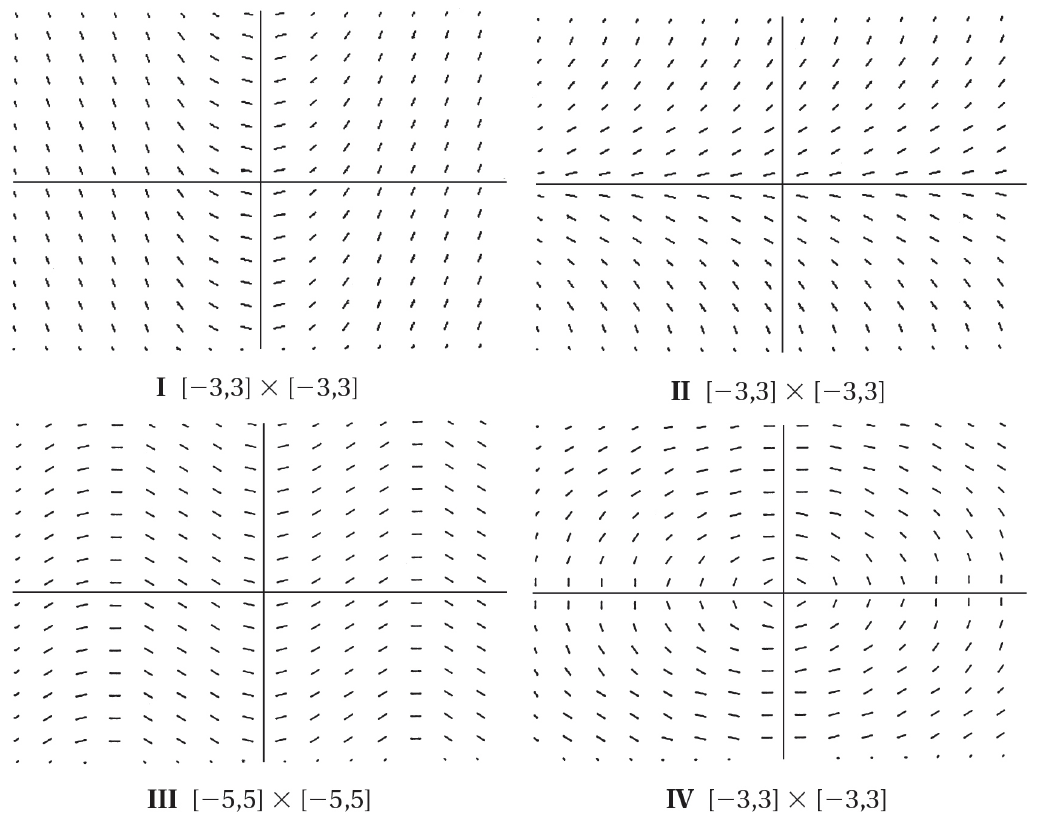
\includegraphics[width=0.6\linewidth]{data/calculus-figures/c9-a25-a29.png}\end{center}
\begin{list}{}{\setlength{\leftmargin}{3em}\setlength{\labelwidth}{2.5em}\setlength{\itemsep}{0pt}\setlength{\topsep}{2pt}}
\item[(A)] $y=-e^x$
\item[(B)] $y=-e^{-x}$
\item[(C)] $y=x^2-1$
\item[(D)] $y=-\cos x$
\end{list}

\bigskip\noindent\textbf{A30.}\ Use Euler's method with step $0.1$ for $y'=x$, $y(1)=5$, to estimate $y(1.2)$.
\begin{list}{}{\setlength{\leftmargin}{3em}\setlength{\labelwidth}{2.5em}\setlength{\itemsep}{0pt}\setlength{\topsep}{2pt}}
\item[(A)] $5.10$
\item[(B)] $5.20$
\item[(C)] $5.21$
\item[(D)] $6.05$
\end{list}

\bigskip\noindent\textbf{A31.}\ For $y'=x$ and $y(1)=5$, Euler's method with step $0.1$ estimates $y(1.2)$ as $5.21$. What is the absolute error?
\begin{list}{}{\setlength{\leftmargin}{3em}\setlength{\labelwidth}{2.5em}\setlength{\itemsep}{0pt}\setlength{\topsep}{2pt}}
\item[(A)] $0.005$
\item[(B)] $0.010$
\item[(C)] $0.050$
\item[(D)] $0.500$
\end{list}

\bigskip\noindent\textbf{A32.}\ Which differential equation has the displayed slope field?
\begin{center}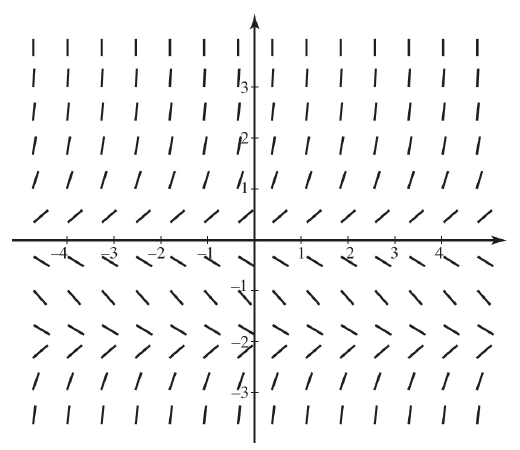
\includegraphics[width=0.6\linewidth]{data/calculus-figures/c9-a32.png}\end{center}
\begin{list}{}{\setlength{\leftmargin}{3em}\setlength{\labelwidth}{2.5em}\setlength{\itemsep}{0pt}\setlength{\topsep}{2pt}}
\item[(A)] $y'=y(y+2)$
\item[(B)] $y'=xy+2$
\item[(C)] $y'=x/(y+2)$
\item[(D)] $y'=y/(y+2)$
\end{list}

\bigskip\noindent\textbf{A33.}\ Which function can solve the displayed slope field?
\begin{center}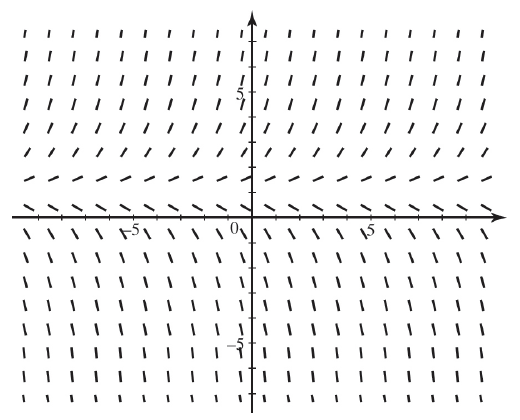
\includegraphics[width=0.6\linewidth]{data/calculus-figures/c9-a33.png}\end{center}
\begin{list}{}{\setlength{\leftmargin}{3em}\setlength{\labelwidth}{2.5em}\setlength{\itemsep}{0pt}\setlength{\topsep}{2pt}}
\item[(A)] $y=1-\ln x$
\item[(B)] $y=1+\ln x$
\item[(C)] $y=1+e^x$
\item[(D)] $y=1+\tan x$
\end{list}

\bigskip\noindent\textbf{A34.}\ Which differential equation has the displayed field on $[-10,10]\times[-7,7]$?
\begin{center}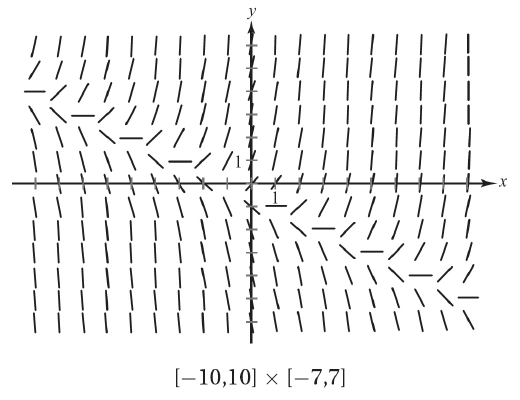
\includegraphics[width=0.6\linewidth]{data/calculus-figures/c9-a34.png}\end{center}
\begin{list}{}{\setlength{\leftmargin}{3em}\setlength{\labelwidth}{2.5em}\setlength{\itemsep}{0pt}\setlength{\topsep}{2pt}}
\item[(A)] $y'=x^2+2y^2+1$
\item[(B)] $y'=2y+1$
\item[(C)] $y'=x-2y+1$
\item[(D)] $y'=x+2y+1$
\end{list}

\bigskip\noindent\textbf{A35.}\ Which differential equation has the displayed field on $[-10,10]\times[-7,7]$?
\begin{center}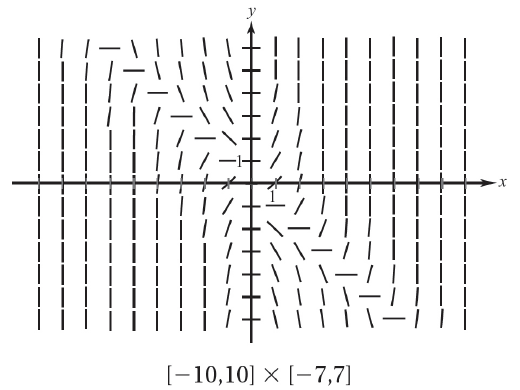
\includegraphics[width=0.6\linewidth]{data/calculus-figures/c9-a35.png}\end{center}
\begin{list}{}{\setlength{\leftmargin}{3em}\setlength{\labelwidth}{2.5em}\setlength{\itemsep}{0pt}\setlength{\topsep}{2pt}}
\item[(A)] $y'=x(x+y)$
\item[(B)] $y'=y(x+y)$
\item[(C)] $y'=x(x+1)$
\item[(D)] $y'=x(x^2+y)$
\end{list}

\bigskip\noindent\textbf{A36.}\ Which differential equation has the displayed field on $[-10,10]\times[-4,4]$?
\begin{center}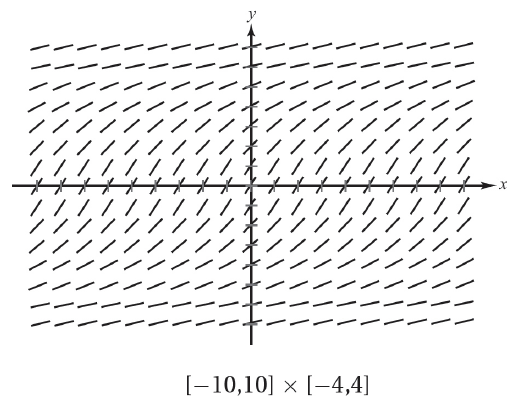
\includegraphics[width=0.6\linewidth]{data/calculus-figures/c9-a36.png}\end{center}
\begin{list}{}{\setlength{\leftmargin}{3em}\setlength{\labelwidth}{2.5em}\setlength{\itemsep}{0pt}\setlength{\topsep}{2pt}}
\item[(A)] $y'=2x/(2+y^2)$
\item[(B)] $y'=2/(2+x^2)$
\item[(C)] $y'=2y/(2+y^2)$
\item[(D)] $y'=2/(2+y^2)$
\end{list}

\bigskip\noindent\textbf{B1.}\ If $ds/dt=\sin^2(\pi s/2)$ and $s(0)=1$, find $t$ when $s=3/2$.
\begin{list}{}{\setlength{\leftmargin}{3em}\setlength{\labelwidth}{2.5em}\setlength{\itemsep}{0pt}\setlength{\topsep}{2pt}}
\item[(A)] $1/2$
\item[(B)] $\pi/2$
\item[(C)] $2/\pi$
\item[(D)] $-2/\pi$
\end{list}

\bigskip\noindent\textbf{B2.}\ If radium decomposes at a rate proportional to the amount present, then the amount $R$ left after $t$ years, if $R_0$ is present initially and $k$ is the negative constant of proportionality, is given by
\begin{list}{}{\setlength{\leftmargin}{3em}\setlength{\labelwidth}{2.5em}\setlength{\itemsep}{0pt}\setlength{\topsep}{2pt}}
\item[(A)] $R=R_0 kt$
\item[(B)] $R=R_0 e^{kt}$
\item[(C)] $R=e^{R_0 kt}$
\item[(D)] $R=e^{R_0+kt}$
\end{list}

\bigskip\noindent\textbf{B3.}\ Population grows at a rate proportional to its current size and doubles in 50 years. Find $P/P_0$ after 75 years.
\begin{list}{}{\setlength{\leftmargin}{3em}\setlength{\labelwidth}{2.5em}\setlength{\itemsep}{0pt}\setlength{\topsep}{2pt}}
\item[(A)] $9/4$
\item[(B)] $5/2$
\item[(C)] $4$
\item[(D)] $2\sqrt2$
\end{list}

\bigskip\noindent\textbf{B4.}\ A substance decays at a rate proportional to its amount, falling from 40 g to 10 g in 2 hours. Find the proportionality constant.
\begin{list}{}{\setlength{\leftmargin}{3em}\setlength{\labelwidth}{2.5em}\setlength{\itemsep}{0pt}\setlength{\topsep}{2pt}}
\item[(A)] $-\ln2$
\item[(B)] $-1/2$
\item[(C)] $-1/4$
\item[(D)] $\ln(1/4)$
\end{list}

\bigskip\noindent\textbf{B5.}\ If $(g'(x))^2=g(x)$ for every real $x$, $g(0)=0$, and $g(4)=4$, find $g(1)$.
\begin{list}{}{\setlength{\leftmargin}{3em}\setlength{\labelwidth}{2.5em}\setlength{\itemsep}{0pt}\setlength{\topsep}{2pt}}
\item[(A)] $1/4$
\item[(B)] $1/2$
\item[(C)] $2$
\item[(D)] $4$
\end{list}

\bigskip\noindent\textbf{B6.}\ The solution of $y'=y$ through $(2,3)$ is
\begin{list}{}{\setlength{\leftmargin}{3em}\setlength{\labelwidth}{2.5em}\setlength{\itemsep}{0pt}\setlength{\topsep}{2pt}}
\item[(A)] $y=e^x+3$
\item[(B)] $y=0.406e^x$
\item[(C)] $y=e^x-(e^2+3)$
\item[(D)] $y=e^x/0.406$
\end{list}

\bigskip\noindent\textbf{B7.}\ Where a solution of $y'=x+y$ intersects $x+y=0$, the function
\begin{list}{}{\setlength{\leftmargin}{3em}\setlength{\labelwidth}{2.5em}\setlength{\itemsep}{0pt}\setlength{\topsep}{2pt}}
\item[(A)] equals zero
\item[(B)] has a local maximum
\item[(C)] has a local minimum
\item[(D)] has an inflection point
\end{list}

\bigskip\noindent\textbf{B8.}\ The graph shows the slope field $F'(x)=e^{-x^2}$ and solution $F(0)=0$. Find $\lim_{x\to\infty}F(x)$ to three decimals.
\begin{center}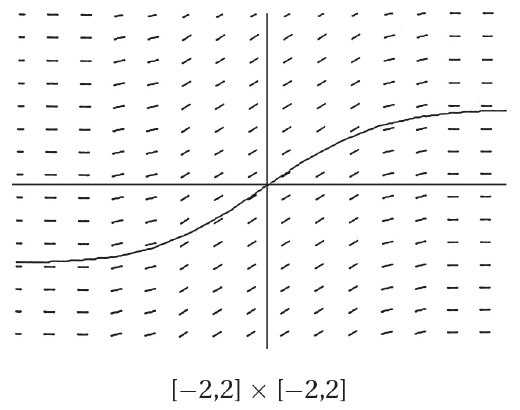
\includegraphics[width=0.6\linewidth]{data/calculus-figures/c9-b8.png}\end{center}
\begin{list}{}{\setlength{\leftmargin}{3em}\setlength{\labelwidth}{2.5em}\setlength{\itemsep}{0pt}\setlength{\topsep}{2pt}}
\item[(A)] $0.886$
\item[(B)] $0.987$
\item[(C)] $1.000$
\item[(D)] $\infty$
\end{list}

\bigskip\noindent\textbf{B9.}\ The graph shows logistic growth of frog population $F$ toward 1000. Which equation models it?
\begin{center}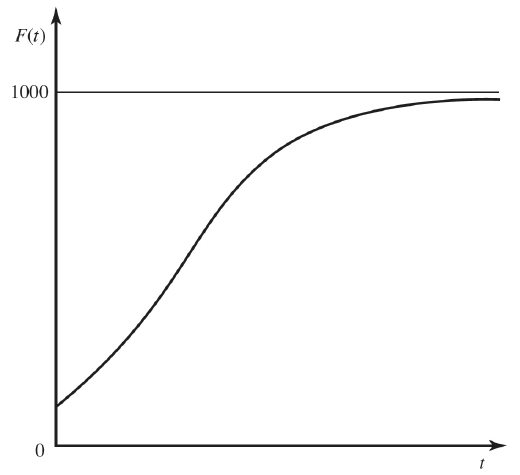
\includegraphics[width=0.6\linewidth]{data/calculus-figures/c9-b9.png}\end{center}
\begin{list}{}{\setlength{\leftmargin}{3em}\setlength{\labelwidth}{2.5em}\setlength{\itemsep}{0pt}\setlength{\topsep}{2pt}}
\item[(A)] $F'=1.5F-0.003F^2$
\item[(B)] $F'=1.5F^2-0.003F$
\item[(C)] $F'=3F-0.003F^2$
\item[(D)] $F'=0.003F^2-3F$
\end{list}

\bigskip\noindent\textbf{B10.}\ The derivative table is $\begin{array}{c|rrrrrr}x&2&3&4&5&6&7\\\hline f\prime(x)&2&2.5&1&-0.5&-1.5&0.5\end{array}$. Given $f(3)=100$, use Euler's method with step $2$ to estimate $f(7)$.
\begin{list}{}{\setlength{\leftmargin}{3em}\setlength{\labelwidth}{2.5em}\setlength{\itemsep}{0pt}\setlength{\topsep}{2pt}}
\item[(A)] $102.5$
\item[(B)] $103$
\item[(C)] $104$
\item[(D)] $104.5$
\end{list}

\bigskip\noindent\textbf{B11.}\ Coffee initially at $180^\circ$F cools in a $68^\circ$F room according to $y'=-0.11(y-68)$. Find its temperature after 10 minutes.
\begin{list}{}{\setlength{\leftmargin}{3em}\setlength{\labelwidth}{2.5em}\setlength{\itemsep}{0pt}\setlength{\topsep}{2pt}}
\item[(A)] $96$
\item[(B)] $100$
\item[(C)] $105$
\item[(D)] $110$
\end{list}

\bigskip\noindent\textbf{B12.}\ Coffee initially at $180^\circ$F cools in a $68^\circ$F room according to $y'=-0.11(y-68)$. About how many minutes until it reaches $75^\circ$F?
\begin{list}{}{\setlength{\leftmargin}{3em}\setlength{\labelwidth}{2.5em}\setlength{\itemsep}{0pt}\setlength{\topsep}{2pt}}
\item[(A)] $15$
\item[(B)] $18$
\item[(C)] $20$
\item[(D)] $25$
\end{list}

\bigskip\noindent\textbf{B13.}\ Medication concentration drops at a rate proportional to its current concentration, with proportionality factor 30 percent per hour. About how many hours until one-tenth remains?
\begin{list}{}{\setlength{\leftmargin}{3em}\setlength{\labelwidth}{2.5em}\setlength{\itemsep}{0pt}\setlength{\topsep}{2pt}}
\item[(A)] $3$
\item[(B)] $4\tfrac13$
\item[(C)] $6\tfrac23$
\item[(D)] $7\tfrac23$
\end{list}

\bigskip\noindent\textbf{B14.}\ Which of the following statements characterize(s) the logistic growth of a population whose limiting value is $L$ and whose initial value is less than $\dfrac{L}{2}$?

 I. The growth rate initially increases. II. The growth rate is maximal at population $L/2$. III. The growth rate tends to zero as population tends to $L$.
\begin{list}{}{\setlength{\leftmargin}{3em}\setlength{\labelwidth}{2.5em}\setlength{\itemsep}{0pt}\setlength{\topsep}{2pt}}
\item[(A)] I only
\item[(B)] I and II only
\item[(C)] II and III only
\item[(D)] I, II, and III
\end{list}

\bigskip\noindent\textbf{B15.}\ Which differential equation is not logistic?
\begin{list}{}{\setlength{\leftmargin}{3em}\setlength{\labelwidth}{2.5em}\setlength{\itemsep}{0pt}\setlength{\topsep}{2pt}}
\item[(A)] $P'=P-P^2$
\item[(B)] $y'=0.01y(100-y)$
\item[(C)] $x'=0.8x-0.004x^2$
\item[(D)] $R'=0.16(350-R)$
\end{list}

\bigskip\noindent\textbf{B16.}\ An animal population satisfies $P'=0.002P(1000-P)$ with $P(0)=200$. When is it growing fastest?
\begin{list}{}{\setlength{\leftmargin}{3em}\setlength{\labelwidth}{2.5em}\setlength{\itemsep}{0pt}\setlength{\topsep}{2pt}}
\item[(A)] Initially
\item[(B)] When $P=500$
\item[(C)] When $P=1000$
\item[(D)] When $P''>0$
\end{list}

\end{document}
